\chapter{Heat}

Let's say you put a 1 kg aluminum pan that is $80^\circ$ C into
3 liters of water that is $20^\circ$ C. Energy, in the form of heat,
will be transferred from the pan to the water until they are at the same
temperature. (We call this ``thermal equilibrium.'')\index{thermal equilibrium}

What will the temperature of the water be?

\section{Specific Heat Capacity}

If you are heating something, the amount of energy you need to
transfer to it depends on three things: the mass of the thing you are
heating, the amount of temperature change you want, and the
\textit{specific heat capacity} of that substance.\index{specific heat capacity}

\begin{mdframed}[style=important, frametitle={Energy in Heat Transfer}]

  The energy moved in a heat transfer is given by

  $$E = m c \Delta_T$$

  where $m$ is the mass, $\Delta_T$ is the change in temperature, and
  $c$ is the specific heat capacity of the substance.
% ADD: q=mcat

  (Note that this
  assumes no phase change. For example, this formula works nicely on
  warming liquid water, but it gets more complicated if you warm the
  water past its boiling point.)

\end{mdframed}

Can we guess the specific heat capacity of a substance? It is very,
very difficult to guess the specific heat of a substance, so we determine
it by experimentation.

For example, someone determined that it took about 0.9 joules to raise
the temperature of solid aluminum one degree Celsius. So we say ``The
specific heat capacity of aluminum is 0.9 J/g $^\circ$C.''

The specific heat capacity of liquid water is about 4.2 J/g $^\circ$C.

To answer the question, then, the amount of energy given off by the
pan must equal the amount of energy absorbed by the water. And they
need to be the same temperature at the end.  Let $T$ be the final
temperature of both.

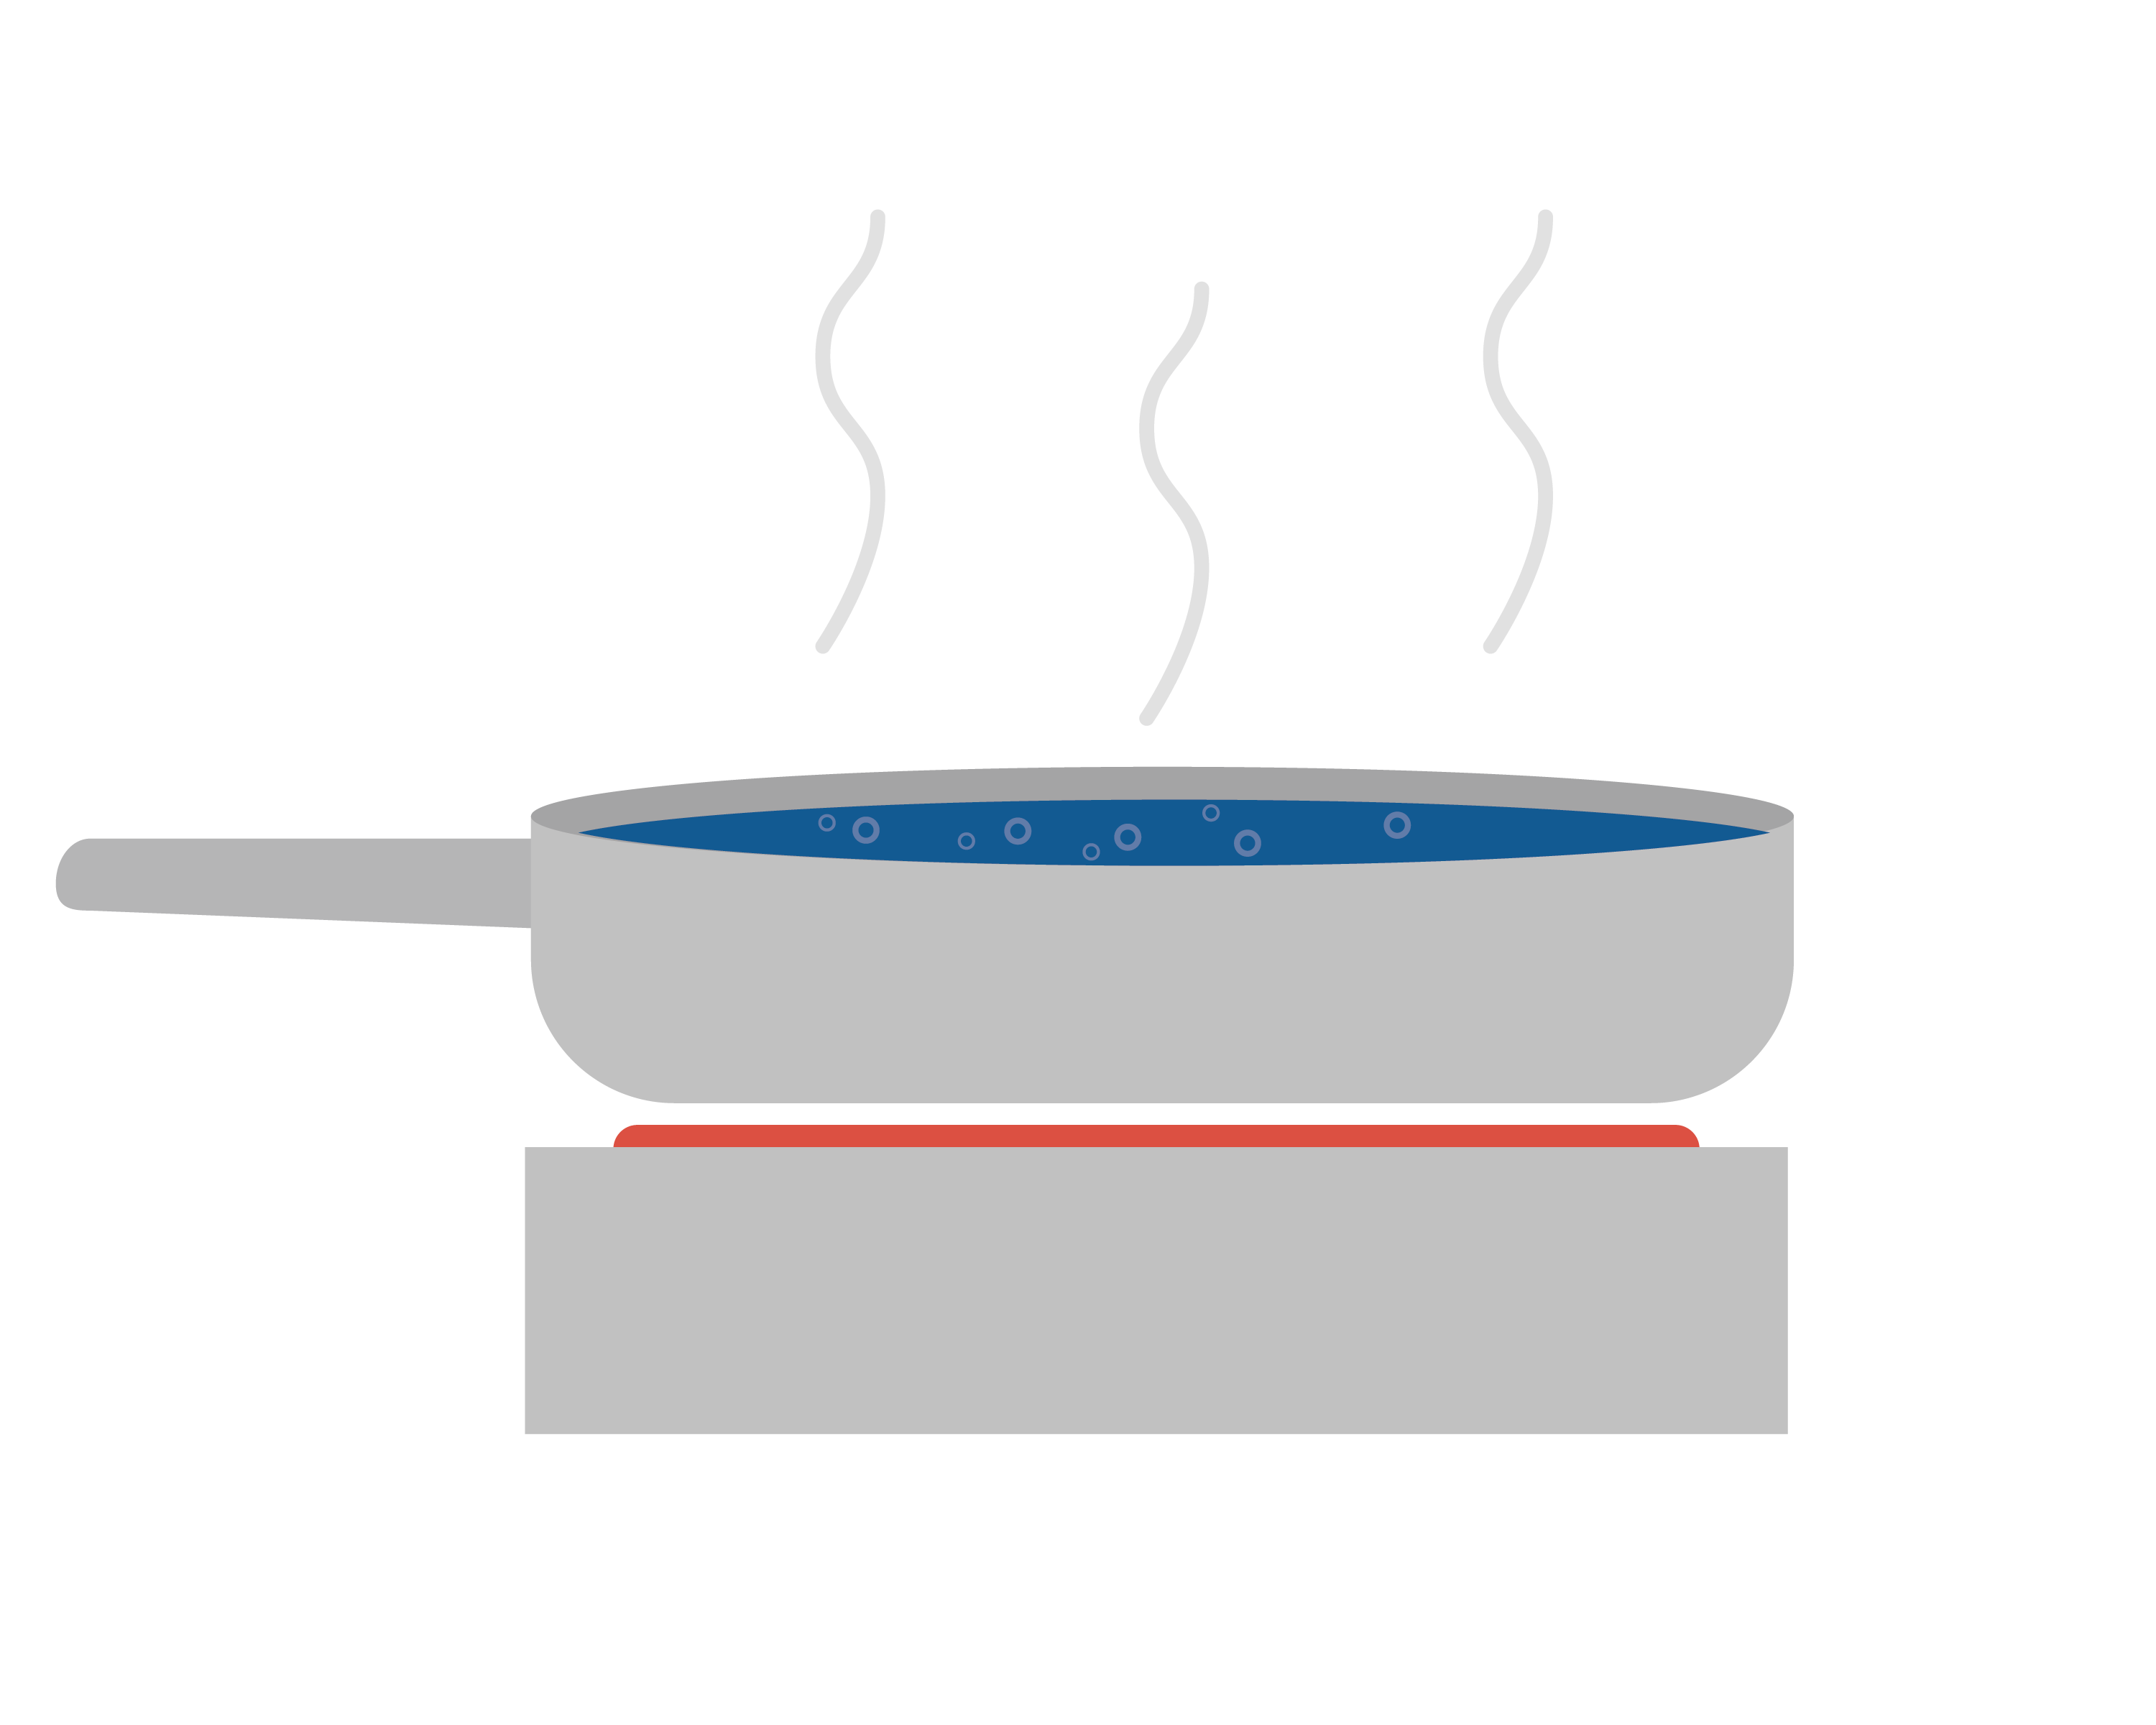
\includegraphics[width=0.5\textwidth]{pan.png}

Watch Khan Academy's discussion of heat capacity at \url{https://www.khanacademy.org/science/ap-chemistry-beta/x2eef969c74e0d802:thermodynamics/x2eef969c74e0d802:heat-capacity-and-calorimetry/v/heat-capacity}


Three liters of water weighs 3,000 grams, so the
change in energy in the water will be:

$$E_W = m c \Delta_T = (3000)(4.2)(T - 20) = 12600T - 252000 \text{ joules}$$ 

The pan weighs 1000 grams, so the change in energy in the pan will be::

$$E_P = m c \Delta_T = (1000)(0.9)(T - 80) = 900T - 72000 \text{ joules}$$

Total energy stays the same so $E_W + E_P = 0$.  So you need to solve

$$(12600T - 252000) + (900T - 72000) = 0$$

And find that the temperature at equilibrium will be

$$T = 24^\circ \text{C}$$

\begin{Exercise}[title={Thermal Equilibrium}, label=thermal_equilibrium]

Just as you put the aluminium pan in the water as described above,
someone also puts a 1.2 kg block of copper cooled to 10 $^\circ$ C.
The specific heat of solid copper is about 0.4 J/g $^\circ$C.

What is the new temperature at equilibrium?

\end{Exercise}
\begin{Answer}[ref=thermal_equilibrium]

  $$E_C = (1200)(0.4)(T - 10) = 480T - 4800$$

Total energy stays constant:

$$0 = (12600T - 252000) + (900T - 72000) + (480T - 4800)$$

Solving for $T$ gets you $T = 23.52^\circ$ C.

\end{Answer}

\section{Getting to Equilibrium}

When two objects with different temperatures are touching, the speed
at which they exchange heat is proportional to the differences in
their temperatures. Thus, as their temperatures get closer together,
the heat exchange slows down.
% ADD: explain which object, water or metal has a greater tempature change

In our example, the pan and the water will get close to equilibrium
quickly, but they may never actually reach equilibrium.

\begin{tikzpicture}
    \begin{axis}[
        xmin=0,xmax=4.25,
        ymin=15,ymax=85,
        axis x line=middle,
        axis y line=middle,
        axis line style=<->,
        xlabel={minutes},
        ylabel={degrees celsius},
        ]
        \addplot[no marks,sdkblue] expression[domain=0:4,samples=100]{24 + 56 * pow(2,-1.5 * x)} node[above, xshift=-1cm, yshift=0.1cm]{Pan}; 
        \addplot[no marks,sdkblue] expression[domain=0:4,samples=100]{24 - 4 * pow(2,-0.8 * x)} node[below, xshift=-2.5cm]{Water};
        \addplot[no marks,dashed,gray] coordinates {(0,24)(6,24)} node[above, xshift=-8cm]{equilibrium};
    \end{axis}
\end{tikzpicture}

\begin{Exercise}[title={Cooling Your Coffee}, label=cool_coffee]

  You have been given a ridiculously hot cup of coffee and a small pitcher of chilled milk.

  You need to start chugging your coffee in three minutes, and you want it as cool as possible at that time. When should you add the milk to the coffee?

\end{Exercise}
\begin{Answer}[ref=cool_coffee]

  During the 3 minutes, you want the coffee to give off as much of its
  heat as possible, so you want to maximize the difference between the
  temperature of the coffee and the temperature of the room around
  it.

  You wait until the last moment to put the milk in.

\end{Answer}

\section{Specific Heat Capacity Details}

For any given substance, the specific heat capacity often changes a
lot when the substance changes state. For example, ice is 2.1 J/g
$^\circ$C, whereas liquid water is 4.2 J/g$^\circ$C.

Watch Khan Academy's discussion of the specific heat of water: \url{https://www.khanacademy.org/science/biology/water-acids-and-bases/water-as-a-solid-liquid-and-gas/v/specific-heat-of-water}

Even within a given state, the specific heat capacity varies a bit
based on the temperature and pressure. If you are trying to do these
sorts of calculations with great accuracy, you will want to find the
specific heat capacity that matches your situation. For example, I
might look for the specific heat capacity for water at $22^\circ$C at
1 atmosphere of pressure( atm).

